\clearpage
\section{Test Results - Black Box Testing}

In this section we will give a summary of the results. The full vulnerability report is in a separate document (“Vulnerability Reporting Form”) and will contain more information.

\subsection{OWASP-AT-001 - Credentials Transported Over an Encrypted Channel}
The website does not use SSL. We can see that in the header that the page uses only HTTP and not 
HTTPS. This is often critical on pages where there is transfer of sensitive data.

\subsection{OWASP-AT-002 - User Enumeration and Guessable User Accounts}
When a user is typing an email or a password, the website responds if the email or password is correct. If you type an email, and the email already exists, the user will get a message that the password was wrong. This means that an intruder can get information about registered users and then bruteforce passwords to get in. In the pictures you can see that we have tried an email, then a password. The website gives us the information that the email is actually a registered user, but the password is incorrect.


\begin{figure}[!ht]
\begin{subfigure}{.5\textwidth}
  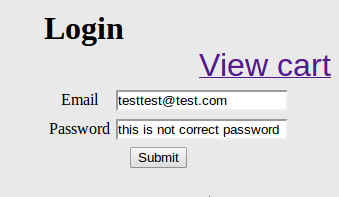
\includegraphics[scale=0.5]{pics/login1.png}
\end{subfigure}%
\begin{subfigure}{.5\textwidth}
  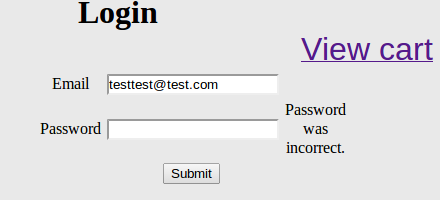
\includegraphics[scale=0.5]{pics/login2.png}
\end{subfigure}
\end{figure}

\subsection{OWASP-AT-003 - Default or Guessable Users/Passwords}There is no password policy at the page, i.e., you are not alerted if your password is weak. It is also possible to make an “empty” password (no password at all). It did not take a lot of time guessing for users and passwords, but we can clearly see that this is a vulnerable point. A site without any password policy is easier to bruteforce than a site with a password policy with more complex passwords to crack.
The point previously mentioned is that the site will give you a clue if you have entered some of the information connected to a registered user. We managed to guess a test user’s name of the system - test@test.com. Using WebCruiser we also got access to default account (WCRTESTINPUT000000 / WCRTESTINPUT000002).

\subsection{OWASP-AT-004 - Bruteforce}Since the page allows us to get information if the user is registered, it would be an easier task to do a brute force attack. We used a tool called “Brutus” without success. As possible users name we wrote users, that we found out exist, as dictionary for passwords we wanted to try first the default one. It returned us some passwords, but all of them were wrong.
Also, since we managed to breach the whole database, we tried to get password out of Hash. Hash used there is 40 symbols long and that looks like either the SHA-1 algorithm was used or MySQL5. We set up RainbowCrack software and created rainbow chaines for SHA-1 algorithm, but it could not decrypt our hashes. We also tried to decrypt the hash using web-services and found one site, where they could get almost every password staying behind hash, but we were supposed to pay a small amount for this service. 

\subsection{OWASP-AT-005 - Bypassing}
On a webpage there are some sites that needs authentication to get access. Bypassing means getting access to pages that you should not get access to by not going through any authentication at all.
On the pagemap we made, we have certain pages that require authentication to access. One way we tried to do a bypass was by entering the authentication sites with direct page request (forced browsing), but it didnt work. We also tried to do some SQL injections to get access, but we didnt succeed with that without using any tools. 

\subsection{OWASP-AT-006 - Stored Password and Password Reset}
The only way to store the password is to keep the browser open because the cookie that contains the sessionID lives as long as the browser is open. There is also no way to “log out” without closing the browser. If you forget your password, there is no “function” to restore your password, so we didn’t get the chance to test that.

\subsection{OWASP-SM-001 - Session Management Schema}
We managed to obtain cookie information such as the fact that there’s only one. It is highly persistent (never close the browser, never delete the cookie). The cookie operations are not performed over encrypted transport. We did not manage to fake a valid cookie.

\subsection{OWASP-SM-002 - Cookies Attributes}
By getting a cookie-ID via CSRF it is easy to steal another user’s account information. It is enough to simply install a plugin that allows to change the cookie-value to the one that was sent. By doing this we managed to log in as another person without him knowing it.

\subsection{OWASP-SM-003 - Session Hijacking}
Using Javascript, we created a redirection to a different web-page (supposed to be a hacker’s website) with cookie as a GET-parameter. The hacker’s webpage is supposed to take this information and present it to the hacker. By doing this we managed to hijack the session of another user and be logged in as him/her.

\subsection{OWASP-SM-004 - Exposed Session Variables}
We looked up the stored cookie, which was a session cookie with the expire information “when the browser is closed”, and the ID right there. Still, we did not have time to see if there is any reuse, or close to reuse (predictable) session tokens.

\subsection{OWASP-SM-005 - CSRF}
Using Javascript injected through the Complaints-page, wrote a script that selects a random picture from Flickr and posts it to the mail log on behalf of whomever is logged into the bookstore. This happens every time someone visits the Mail Log-page.

\begin{figure}[!ht]
	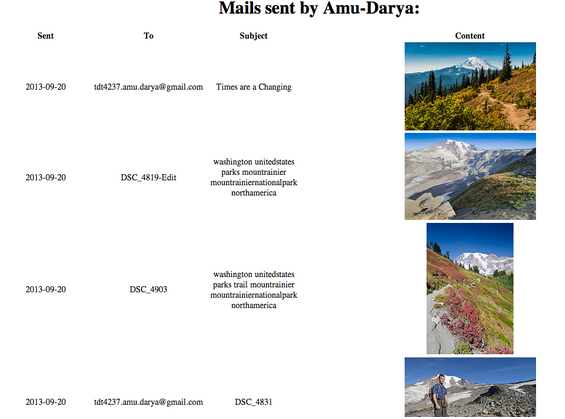
\includegraphics[scale=0.8]{pics/testtest3.png}
\end{figure}

\subsection{OWASP-AZ-001 - Path Traversal}
We read all the URLs and we noticed certain ones that might be exploited, but we did not manage to do so. Therefore we don’t know whether they are actually exposable. We might have misread the (non-existing) opportunity, or we could have overlooked one.

\subsection{OWASP-BL-001 - Business Logic}
A flaw in the business logic was discovered. There is no data validation of the user input on the book ordering page. This means that a user is able to order a negative quantity of books. The user is therefore able to order books, and then order a negative quantity of a different book, giving him-/herself “store credit”. It is also possible that a user may only order a negative quantity of books. If the circumstances are right, and the source code is set up in a certain way, this might lead to the user actually making money, simply by hitting the order button.

\begin{figure}[!ht]
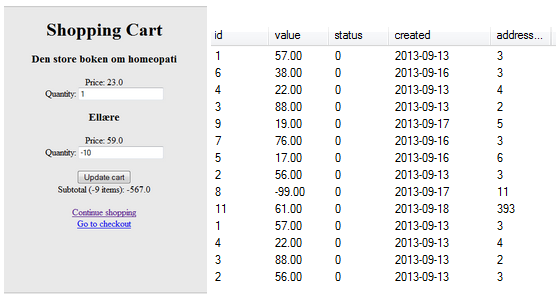
\includegraphics[scale=0.7]{pics/testtest4.png}
\end{figure}

Above, on the left, we can see that a user has succsessfully added a negative quantity of books. On the right we are able to see that the table “Order” in the websites’ database stores the values as negative numbers (-99.00). 

\subsection{OWASP-DV-001 - Reflected Cross Site Scripting}
We discovered a possibility to make a script in a form under the complaints page. When a user submits a complaint, the complaint is posted in the email log. When entering the email log site, all the complaints are displayed, and also the scripts submitted by regular users are running in the background. We tried with a friendly annoying script with a pop-up alert message. This is not doing any harm and the user is notified, but we can also make scripts that are running in the background without the user knowing. We also tried to add a script that added a cookie, and it worked. We have not made the cookie to do any harm, but this is possible. 

\begin{figure}[!ht]
\begin{subfigure}{.5\textwidth}
  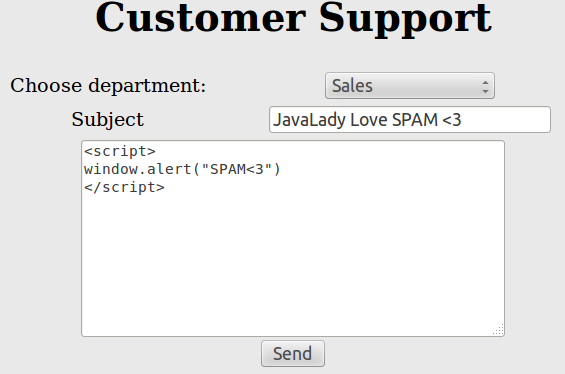
\includegraphics[scale=0.3]{pics/screen3.png}
\end{subfigure}%
\begin{subfigure}{.5\textwidth}
  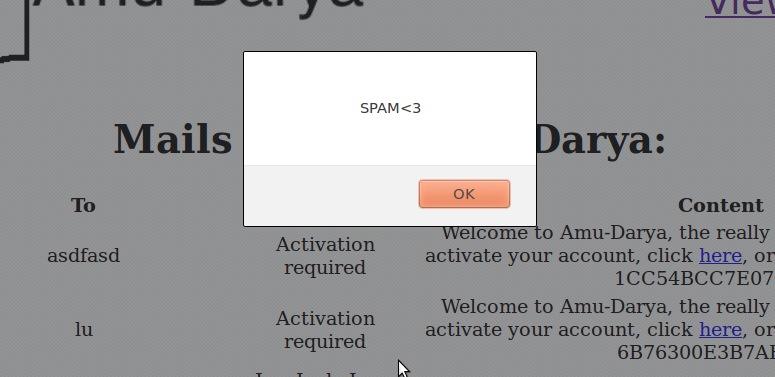
\includegraphics[scale=0.3]{pics/screen4.png}
\end{subfigure}
\end{figure}

\subsection{OWASP-DV-005 - SQL Injection}
We have used a tool called WebCruiser to do a vulnerability scan. During the scan the program found a vulnerability in the book information page. It used SQL injection and got access to the database structure as well as the data. We can clearly see that there is a lot of sensitive data stored that we now have access to; e.g., password, username, creditcard, etc.

We also made SQL injections in other places. It is possible to write an SQL injection in the email-field and we made a SQL URL- injection in ViewBook. Here we could select another book depending on what we want, e.g. price, isbn13 or other fields. We tried to join the query with another table and get credit card information instead, but were not able to guess the structure of the original query. We managed to prove SQL vulnerability in most fields, but didn’t manage an exploit. \#, “); and foo” or ‘1=1 was accepted, but SQL injection more complex than that was only done by the tool.

{\bf The Database Structure:}
\begin{itemize}
	\item {\bf book:} (id, title\textunderscore id, edition, price, isbn13, binding, isbn10, published, publisher\textunderscore id, des)
	\item {\bf address} (id, address, customer\textunderscore id)
	\item {\bf author:} (id, name)
	\item {\bf category}
	\item {\bf mail:} (id, to, subject, content, sentTime)
	\item {\bf customer:} (id, email, name, password, activation\textunderscore token)
	\item {\bf title:} (id, name)
	\item {\bf credit\textunderscore card:} (id, cc\textunderscore number, customer\textunderscore id, expiry\textunderscore date, cardholder\textunderscore name)
	\item {\bf author\textunderscore x\textunderscore book}
	\item {\bf order\textunderscore items}
	\item {\bf publisher}
	\item {\bf category\textunderscore x\textunderscore title}
	\item {\bf .order}
\end{itemize}

\newpage

\subsection{Other Vulnerabilities}
We wanted to check what kind of protocol the server uses to communicate with the client, and found out that is uses the TCP/IP. Using this protocol is more secure, as opposed to e.g., UDP, and is therefor not consideres to be a vulnerability for this application.

When posting a complaint, the client side stores the email it sends it to. By easily editing the email address in the HTML in the web browser, we managed to send the email to ourselves instead of the predefined recipient.

\begin{figure}[!ht]
  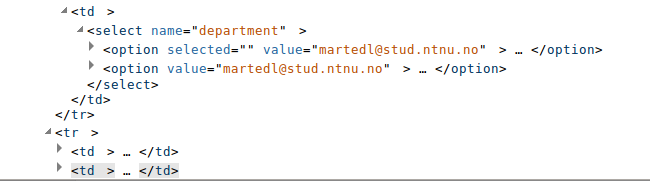
\includegraphics[scale=0.5]{pics/screen7.png}
  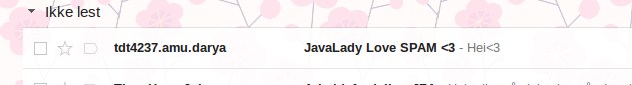
\includegraphics[scale=0.5]{pics/screen8.png}
\end{figure}

We managed to manipulate parameters with Fiddler. We tried to change the total price of the order. It is possible if the breakpoint after the response from server is set, but since the bookstore only sends book ID and quantity to server, it was not possible to change the price of an item. By changing the total price on the client side we were not able to make it store the wrong value on an order in the database.

\begin{figure}[!ht]
	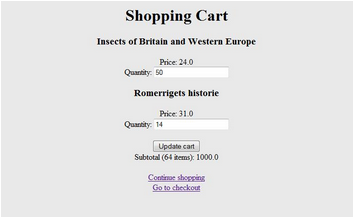
\includegraphics[scale=0.8]{pics/testtest2.png}
\end{figure}

\begin{figure}[!ht]
	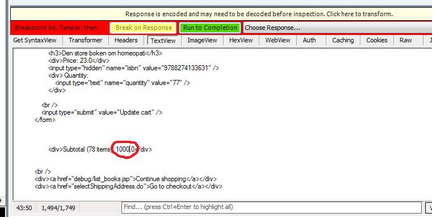
\includegraphics[scale=0.8]{pics/testtest.png}
\end{figure}
